%%%%%%%%%%%%%%%%%%%%%%%%%%%%%%%%%%%%%%%%%
% TMDEI Dissertation
% LaTeX Template
% Version 0.1 (Dec/2015)
%
% Adapted to TMDEI/ISEP style (Dec/2015) by
%  Nuno Pereira (nap@isep.ipp.pt) and
%  Paulo Baltarejo (pbs@isep.ipp.pt)
%
% Based on MastersDoctoralThesis Version 1.2 by Vel (vel@latextemplates.com) and
% Johannes Böttcher, downloaded from (21/11/15):
% http://www.LaTeXTemplates.com
%
% This template is originally based on a template by:
% Steve Gunn (http://users.ecs.soton.ac.uk/srg/softwaretools/document/templates/)
% Sunil Patel (http://www.sunilpatel.co.uk/thesis-template/)
%
% Template license:
% CC BY-NC-SA 3.0 (http://creativecommons.org/licenses/by-nc-sa/3.0/)
%
%%%%%%%%%%%%%%%%%%%%%%%%%%%%%%%%%%%%%%%%%

%----------------------------------------------------------------------------------------
%	PACKAGES AND OTHER DOCUMENT CONFIGURATIONS
%----------------------------------------------------------------------------------------

\documentclass[
11pt, % The default document font size, options: 10pt, 11pt, 12pt
%oneside, % Two side (alternating margins) for binding by default, uncomment to switch to one side (for drafting/reading purposes)
portuguese, % english for English;
%portuguese,% for Portuguese; delete temporary files if you change language (e.g. 'make clean; make')
singlespacing, % Single line spacing, alternatives: onehalfspacing or doublespacing (for drafting/reading purposes)
%draft, % Uncomment to enable draft mode (no pictures, no links, overfull hboxes indicated)
%nolistspacing, % If the document is onehalfspacing or doublespacing, uncomment this to set spacing in lists to single
liststotoc, % Uncomment to add the list of figures/tables/etc to the table of contents (not recommended)
%toctotoc, % Uncomment to add the main table of contents to the table of contents (not recommended)
parskip, % Add space between paragraphs (recommended)
%nohyperref, % Uncomment to not load the hyperref package (not recommended)
nohyperreflinkcolor, % hyperref links are not colored (comment to color links, for example to produce an electronic-only version)
headsepline, % Uncomment to get a line under the header
]{tmdei-style} % The class file specifying the document structure

\usepackage{soul}
\usepackage{tikz} % Required for creating graphics programmatically (can be removed if not used)
%\usetikzlibrary{arrows} % Required for fancy arrows in TiKZ graphics (can be removed if not used)

\usepackage{pgfplots} % Required for drawing high--quality function plots (can be removed if not used)
\pgfplotsset{compat=newest}

%
% Next you have examples of admissable citation styles; we recomend using the authoryear-comp citation style (which resembles Harvard); don't forget to only uncomment one
%

% authoryear-comp: recommended citation style (e.g. (Buendía, 1860), (Buendía 1910, Arcadio 1940))
\usepackage[style=authoryear-comp,backend=biber]{biblatex} % Bibtex backend with the authoryear-comp citation style (authoryear citations, bibliography ordered alphabetically)

% numeric citation style (e.g. [1], [1-3])
%\usepackage[style=numeric-comp,sorting=none,backend=biber]{biblatex} % Bibtex backend with the numeric-comp citation style (numeric citations, bibliography ordered by appearance)

% alphabetic citation style (e.g. [Buendía10], [Buendía10, Arcadio40])
%\usepackage[style=alphabetic,sorting=none,backend=biber]{biblatex} % Bibtex backend with the alphabetic citation style (alphabetic citations, bibliography ordered by appearance)


\addbibresource{mainbibliography.bib} % The filename of the bibliography

\makeglossaries % build the glossary

%----------------------------------------------------------------------------------------
%	THESIS INFORMATION
%----------------------------------------------------------------------------------------

\thesistitle{Natural Language Querying} % Your thesis title, this is used in the title, print it elsewhere with \ttitle

%\thesissubtitle{{[}Thesis Subtitle{]}} % Your thesis title, this is used in the title, print it elsewhere with \tsubtitle

\author{\textsc{Tiago Gabriel da Silva}} % Your name, this is used in the title page, print it elsewhere with \authorname

\subjectarea{Sistemas Computacionais} % Specialization area (Computer Systems, Information and Knowledge Systems, Graphics, Systems and Multimedia, Software Engineering), used in the title page, print it elsewhere with \areaname

\supervisor{Dr. Paulo Gandra da Sousa} % Your supervisor's name, this is used in the title page, print it elsewhere with \supname

\cosupervisor{Eng.º Ricardo \textsc{Magalhães}} % Your co-supervisor's name, this is used in the title page, print it elsewhere with \cosupname (comment, if no co-supervisor)

\committeepresident{Dr. Jonny Smith, Professor, DEI/ISEP} % Name of the president of the evaluation committee, print it elsewhere with \presidentname

\committeemembers{Dr. Jaimie Smith, Professor, DEI/ISEP\\Dr. Jones Smith, Professor, DEI/ISEP\\Dr. Jagger Smith, Professor, DEI/ISEP} % Name of the evaluation committee members (up to four), print it elsewhere with \committee

\keywords{Inteligência Artificial, Linguagem Natural, \textit{Manufacturing Execution Systems}, \textit{Querying}} % Please define up to 6 keywords that better describe your work, print it elsewhere with \keywordnames

\university{\href{http://www.isep.ipp.pt}{Instituto Superior de Engenharia do Porto}} % Your university's name and URL, this is used in the title page and abstract, print it elsewhere with \univname

\department{\href{http://www.dei.isep.ipp.pt}{Departamento de Engenharia Informática}} % Your department's name and URL, this is used in the title page and abstract, print it elsewhere with \deptname

\thesisdate{Porto, \today} % thesis date,  print it elsewhere with \tdate

\hypersetup{pdftitle=\ttitle} % Set the PDF's title to your title
\hypersetup{pdfauthor=\authorname} % Set the PDF's author to your name
\hypersetup{pdfkeywords=\keywordnames} % Set the PDF's keywords to your keywords

\begin{document}

%----------------------------------------------------------------------------------------
%	FRONT MATTER
%----------------------------------------------------------------------------------------

% Include the frontmatter of your thesis here
% we include the glossary here (front matter is included with \input, so this command is as if it was in main.tex)
% Acrónimos
\newacronym{iot}{IoT}{\textit{Internet of Things}}
\newacronym{ios}{IoS}{\textit{Internet of Services}}
\newacronym{ihc}{IHC}{Interação Humano-Computador}
\newacronym{ia}{IA}{Inteligência Artificial}
\newacronym{pln}{PLN}{Processamento de Linguagem Natural}
\newacronym{mes}{MES}{\textit{Manufacturing Execution System}}
\newacronym{sql}{SQL}{\textit{Structured Query Language}}
\newacronym{uml}{UML}{\textit{Unified Modeling Language}}
\newacronym{ceo}{CEO}{\textit{Chief Executive Officer}}
\newacronym{cto}{CTO}{\textit{Chief Technical Officer}}
\newacronym{erp}{ERP}{\textit{Enterprise Resource Planning}}
\newacronym{cps}{CPS}{\textit{Cyber-Physical System}}
\newacronym{ffe}{FFE}{\textit{Fuzzy Front End}}
\newacronym{npd}{NPD}{\textit{New Product Development}}
\newacronym{ncd}{NCD}{\textit{New Concept Development}}
\newacronym{slp}{SLP}{\textit{Single Layer Perceptron}}
\newacronym{ilnbd}{ILNBD}{Interfaces de Linguagem Natural para Bases de Dados}
\newacronym{atn}{ATN}{\textit{Augmented Transition Network}}
\newacronym{xml}{XML}{\textit{Extensible Markup Language}}
% for defining plural form
% \newacronym[shortplural=aa,longplural=letters a]{a}{A}{the a}

\frontmatter % Use roman page numbering style (i, ii, iii, iv...) for the pre-content pages

\pagestyle{plain} % Default to the plain heading style until the thesis style is called for the body content

%----------------------------------------------------------------------------------------
%	TITLE PAGE
%----------------------------------------------------------------------------------------

\maketitlepage

%----------------------------------------------------------------------------------------
%	DEDICATION  (optional)
%----------------------------------------------------------------------------------------
\begin{dedicatory}
\tbd
\end{dedicatory}

%----------------------------------------------------------------------------------------
%	ABSTRACT PAGE
%----------------------------------------------------------------------------------------
\begin{abstract}

O paradigma de interação entre Homem e Máquina tem vindo a mudar nos últimos anos. Se ao longo das últimas décadas, o ser humano tem vindo a interagir com o computador através da escrita (linha de comandos) ou das interfaces gráficas, mais recentemente, surge a interação por linguagem natural. Como potenciar a comunicação entre o Homem e os sistemas usados diariamente, usando linguagem natural? Recorrendo ao Processamento de Linguagem Natural, um campo de estudo ligado à Inteligência Artificial, que pode envolver técnicas de \textit{Machine Learning} ou \textit{Deep Learning}, torna-se possível transformar a linguagem do ser humano numa representação adaptada aos sistemas computacionais. 

A presente tese debruça-se na conceção de uma abordagem que permita a consulta e apresentação de informação contida em armazéns de dados, recorrendo a linguagem natural. Neste âmbito, foi desenvolvido um protótipo que assenta sobre a abordagem conceptualizada. Assim, o intuito final é adaptar e usar a abordagem proposta no desenvolvimento dum módulo de linguagem natural para interface com o {\productname}, procurando aprimorar a usabilidade do sistema.

\end{abstract}

\begin{abstractotherlanguage}
The interaction paradigm between man and machine has been changing in the last years. Over the last decades, humans have been interacting with the computer through writing (command line) or graphical interfaces. Recently, emerges the interaction through natural language. How to enhance the communication between man and the system used on daily basis, by using natural language? The usage of Natural Language Processing, a field of study of Artificial Intelligence, which may involve Machine Learning or Deep Learning techniques, allows the transformation of human language into a representation adapted to computation systems.

This thesis focus on the design of an approach that allows to consult and present information stored in data warehouses, through usage of natural language. As result, a prototype has been developed by putting into practise the conceptualized approach. Thus, the main goal is to adapt and use the suggested approach in the development of a natural language module to interact with the {\productname}, thereby improving the system's usability.

\end{abstractotherlanguage}

%----------------------------------------------------------------------------------------
%	ACKNOWLEDGEMENTS (optional)
%----------------------------------------------------------------------------------------
\begin{acknowledgements}

O trabalho desempenhado ao longo de quase um ano não seria possível sem a presença de várias pessoas, as quais marcam a minha vida todos os dias, e das quais tenho apoio incondicional.

Quero agradecer aos meus pais, pela educação, pelo apoio, pelo incentivo e principalmente, pelos valores que me foram incutidos, que fizeram de mim a pessoa que sou hoje. Alguns anos conturbados passaram e hoje tudo faz sentido -- \textit{I'm in hell without you, cannot cope without you two, shocked at the world that I see}. Obrigado.

Agradeço aos meus amigos, por aturarem as minhas longas \inquotes{palestras}, por me ouvirem, na alegria e na tristeza, e por incentivarem o meu sucesso (por ordem alfabética): Diogo, Egídio, Francisco, Joel, Sérgio, Wilson. Grande abraço.

Para o Diogo, obrigado por seres o \textit{brother from another mother}. Ligeiramente picuinhas, eu sei, mas não precisamos de palavras.

Deixo o meu agradecimento ao Instituto Superior de Engenharia do Porto, em particular aos professores que acompanharam o meu percurso e que foram uma inspiração. 

Agradeço à Critical Manufacturing, em especial ao Engenheiro Ricardo Magalhães, pela incentivo dado neste projeto, pelas ideias e pelos desafios que se demonstraram difíceis, mas que com diálogo foram possíveis alcançar. 

Ainda no contexto Critical Manufacturing, quero também deixar o meu agradecimento a todas as pessoas com quem tive o prazer de trabalhar. Quero deixar um agradecimento especial ao Rui Santos, por ter sido o meu mentor na jornada CMF e por me ter \inquotes{dado asas}. Obrigado pelas longas conversas musicais, técnicas e dos momentos de riso. Com certeza que nos vamos cruzar, especialmente em muitos concertos! \textit{Rock On}!

Ao meu orientador, Doutor Paulo Gandra de Sousa, que confiou em mim e no desempenho deste trabalho, que se demonstrou preocupado quando não dava notícias (peço desculpa, professor) e me ajudou a traçar o caminho seguido neste trabalho.

E, como sou uma pessoa que deixa o melhor para o fim, agradeço à Patrícia, minha amiga, confidente, apoiante número um, psicóloga e ouvinte nas horas vagas. Sempre acreditaste em mim, e continuas a fazê-lo, e não há palavras suficientes para descrever a minha gratidão -- \textit{Love of my Life}.

A todos, o meu mais profundo obrigado!
\end{acknowledgements}

%----------------------------------------------------------------------------------------
%	LIST OF CONTENTS/FIGURES/TABLES PAGES
%----------------------------------------------------------------------------------------

\tableofcontents % Prints the main table of contents

\listoffigures % Prints the list of figures

\listoftables % Prints the list of tables

% \iflanguage{portuguese}{
% \renewcommand{\listalgorithmname}{Lista de Algor\'itmos}
% }{}
% \listofalgorithms % Prints the list of algorithms
% \addchaptertocentry{\listalgorithmname}

\iflanguage{portuguese}{
\renewcommand{\lstlistlistingname}{Lista de C\'odigo}
\renewcommand{\lstlistingname}{C\'odigo}
}{ 
\renewcommand{\lstlistlistingname}{List of Source Code}
\renewcommand{\lstlistingname}{C\'ode}
}
\lstlistoflistings
\addchaptertocentry{\lstlistlistingname}

%----------------------------------------------------------------------------------------
%	ABBREVIATIONS
%----------------------------------------------------------------------------------------
%\begin{abbreviations}{ll} % Include a list of abbreviations (a table of two columns)
%\textbf{LAH} & \textbf{L}ist \textbf{A}bbreviations \textbf{H}ere\\
%\textbf{WSF} & \textbf{W}hat (it) \textbf{S}tands \textbf{F}or\\
%\end{abbreviations}

%----------------------------------------------------------------------------------------
%	SYMBOLS
%----------------------------------------------------------------------------------------

%\begin{symbols}{lll} % Include a list of Symbols (a three column table)

$a$ & distance & \si{\meter} \\
$P$ & power & \si{\watt} (\si{\joule\per\second}) \\
%Symbol & Name & Unit \\

\addlinespace % Gap to separate the Roman symbols from the Greek

$\omega$ & angular frequency & \si{\radian} \\

\end{symbols}

%----------------------------------------------------------------------------------------
%	ACRONYMS
%----------------------------------------------------------------------------------------

\newcommand{\listacronymname}{List of Acronyms}
\iflanguage{portuguese}{
\renewcommand{\listacronymname}{Lista de Acr\'onimos}
}
% Use GLS
\glsresetall
\printglossary[title=\listacronymname,type=\acronymtype,style=long]

%----------------------------------------------------------------------------------------
%	DONE
%----------------------------------------------------------------------------------------

\mainmatter % Begin numeric (1,2,3...) page numbering
\pagestyle{thesis} % Return the page headers back to the "thesis" style


%----------------------------------------------------------------------------------------
%	MAIN BODY
%----------------------------------------------------------------------------------------

% Include the chapters of the thesis as separate folder for each chapter
% Uncomment the lines as you write the chapters

\chapter{Introdução}
\label{chap:Chapter1}

A indústria desempenha um papel importante na economia mundial. Desde o início da industrialização, fatores como a evolução tecnológica, as forças políticas e económicas, a competitividade de mercado, levam a mudanças no paradigma industrial, as quais se designam de revoluções industriais. A primeira revolução inicia-se com a mecanização dos processos, segue-se a segunda com o uso da energia elétrica e posteriormente a terceira revolução, fruto da digitalização e informatização industrial~\parencite{industry40, modern_industrial_revolution_exit_failure_internal_control_systems}.

Atualmente, num mercado crescentemente competitivo e exigente, a necessidade de inovar, de obter vantagem competitiva e simultaneamente, tornar os processos industriais simples e altamente eficazes, recorrendo às tecnologias mais atuais, abrem caminho a uma nova mudança. O fenómeno da Indústria 4.0 surge como a nova (quarta) revolução industrial, baseando-se nas mais recentes tecnologias, que incluem os sistemas ciber-físicos, a \gls{IoT} e a \gls{IoS}, as quais se baseiam na comunicação através da Internet, permitindo uma interação contínua e partilha de informação entre humanos, entre máquinas e entre o ser humano e máquina~\parencite{complex_view_industry40}. 

A Indústria 4.0 assenta numa variedade de conceitos fundamentais, de diferentes áreas de conhecimento, nomeadamente a noção de \textit{Smart Factory\footnote{Fábrica Inteligente, equipada com sensores, atuadores e sistemas autónomos, permitindo assim um controlo autónomo de processo.}}, a capacidade de auto-organização, através da descentralização dos sistemas produtivos, e a interação entre o mundo físico e o digital~\parencite[Fundamental Concepts, p.240]{industry40}. No entanto, é a capacidade de adaptação à necessidade humana, principalmente a \gls{IHC}, que se pretende explorar com presente trabalho.

Segundo~\textcite[p.1]{natural_language_translation_intersaction_ai_hci}~\inquotes{as áreas de \gls{IA} e Interação Humano-Computador (\gls{IHC}) estão, cada vez mais, a influenciar-se mutuamente. Sistemas amplamente usados como o Google Translate, Facebook Graph Search e RelateIQ escondem a complexidade de sistemas de larga escala de \gls{IA} através de interfaces intuitivas.}\footnote{Tradução livre do autor. No original~\inquotes{The fields of artificial intelligence (AI) and human-computer interaction (HCI) are influencing each other like never before. Widely used systems such as Google Translate, Facebook Graph Search, and RelateIQ hide the complexity of large-scale AI systems behind intuitive interfaces.}.}. Apesar de terem propósitos diferentes, ambas as áreas se complementam, na medida em que se focam na relação entre ser humano e máquina. Se a \gls{IA} tem como objetivo emular o intelecto humano, já a \gls{IHC} foca-se em abordagens empíricas de usabilidade e fatores humanos, que influenciam a forma como os utilizadores interagem com o computador~\parencite{natural_language_translation_intersaction_ai_hci}. 

A capacidade dum sistema interpretar a linguagem dos seres humanos e apresentar a informação de uma forma adequada, principalmente no contexto da Indústria 4.0, destaca-se como um fator impulsionador da adaptabilidade do mundo digital à necessidade humana. Nesse sentido, a área de \gls{PLN}, a qual se debruça na capacidade dos computadores \inquotes{entenderem} a linguagem humana~\parencite[p.1]{applied_natural_language_processing_with_python}, permite construir ferramentas capazes de definir ações, extrair conhecimento dum sistema e apresentá-lo num formato adequado, a partir de conteúdo textual especificado pelo utilizador, de acordo com a sua própria linguagem. 

\section{Problema}
\label{sec:chap1_problem}

O conceito de \gls{MES}, um sistema que, além de gerir as operações dum determinado processo fabril, mantém dados relativos às diversas etapas inerentes ao processo em questão, está intrinsecamente relacionado com a Indústria 4.0. O Critical Manufacturing \gls{MES} é um destes sistemas. Contudo, a sua incapacidade parcial de adaptar-se às características dos utilizadores, torna-o difícil de usar, numa perspetiva de acesso a informação relevante para o processo e de apoio à decisão. Por outras palavras, se o utilizador pretende efetuar uma determinada pesquisa, necessita de conhecer os detalhes da ferramenta a usar, ao invés de simplesmente \inquotes{pedir} (através de texto ou voz) ao sistema que lhe devolva o resultado.

A \textbf{conceção de um módulo de linguagem natural para interface com o Critical Manufacturing \gls{MES}, permitindo a consulta e pesquisa de estados do processo de fabrico}, torna-se importante para o sistema, uma vez que possibilita o utilizador interagir com o sistema de uma forma simples, intuitiva, eficiente e natural, através de escrita.

\section{Objetivos, Âmbito e Pressupostos}
\label{sec:chap1_objectives}
De uma maneira geral, com este trabalho pretende-se desenvolver uma solução baseada em linguagem natural que promova a interação do utilizador com o sistema \gls{MES}. Com o intuito de solucionar o problema enunciado na secção~\ref{sec:chap1_problem}, definem-se os seguintes objetivos:

\begin{enumerate}
    \item
    \label{enum:ch1_objectives_1}
    {
        \textit{Contextualizar o problema numa perspetiva de negócio} -- análise detalhada do problema, as implicações que tem para negócio e para o produto \gls{MES}, descrevendo o valor intrínseco à solução (Capítulo~\ref{chap:Chapter2});
    }
    \item
    \label{enum:ch1_objectives_2}
    {
        \textit{Estudar soluções disponíveis no mercado e/ou bibliotecas de processamento de linguagem natural} -- obtenção de informação da área de conhecimento envolvida, de ferramentas semelhantes e de bibliotecas tipicamente usadas na implementação de tais módulos (Capítulo~\ref{chap:Chapter3});
    }
    \item
    \label{enum:ch1_objectives_3}
    {
        \textit{Definir a solução mais adequada, considerando as diversas opções apresentadas} -- comparação e avaliação das diversas opções identificadas, selecionando a(s) mais adequada(s), justificando essa(s) escolha(s) (Capítulo~\ref{chap:Chapter3});
    }
    \item
    \label{enum:ch1_objectives_4}
    {
        \textit{Especificação da arquitetura do módulo} -- que permita responder aos requisitos definidos e antecipar soluções para possíveis problemas (\hl{a definir...});
    }
    \item
    \label{enum:ch1_objectives_5}
    {
        \textit{Descrever a semântica de domínio} -- identificação dos domínios a explorar e construção de uma base de conhecimento semântico para o módulo (\hl{a definir...});
    }
    \item
    \label{enum:ch1_objectives_6}
    {
        \textit{Desenvolvimento de prova de conceito} -- implementação da solução de acordo com a arquitetura conceptualizada (\hl{a definir...});
    }
    \item
    \label{enum:ch1_objectives_7}
    {
        \textit{Avaliar a qualidade da solução desenvolvida} -- com base nas metodologias de avaliação definidas, concluir acerca da qualidade da solução e do contributo do trabalho para a resolução do problema (\hl{a definir...});
    }
    \item
    \label{enum:ch1_objectives_8}
    {
        \textit{Elaboração da tese escrita} -- como forma de transmitir o conhecimento alcançado durante a elaboração do trabalho.
    }
\end{enumerate}

Embora os objetivos estejam definidos, surge a necessidade de explicitar sucintamente os assuntos que serão ou não abordados, ou seja, qual o âmbito do trabalho e os pressupostos a ter em consideração.

\section{Critérios de Sucesso}
\label{sec:chap1_success_criteria}
\hl{...}

\section{Contribuições Esperadas}
\label{sec:chap1_contribuitions}
\hl{...}

\section{Metodologia de Trabalho}
\label{sec:chap1_methodology}
\hl{...}

\section{Estrutura da Tese}
\label{sec:chap1_structure}
\hl{...}

\chapter{Contexto}
\label{chap:Chapter2}

\textit{A definir}

\section{A Empresa}
\label{sec:chap2_company}

A {\companyname} é uma empresa fundada em 2009, com sede e centro de engenharia na Maia (Porto, Portugal), subsidiárias em Dresden (Alemanha), Suzhou (China), Austin (Estados Unidos da América) e um escritório comercial em Taiwan. O objetivo é proporcionar à indústria uma solução de gestão e controlo de produção, procurando reduzir os custos de produção, flexibilizar para satisfazer a procura e capacitar a organização de uma maior agilidade, visibilidade e fiabilidade~\parencite{cmf_overview}. O compromisso da empresa~\parencite{cmf_overview} foca-se no desenvolvimento de~\inquotes{soluções de vanguarda, indo de encontro aos desafios mais importantes da indústria e disponibilizar à lista crescente de clientes satisfeitos, soluções de elevado valor acrescentado, no prazo e orçamento requerido}\footnote{Tradução livre do autor. No original~\inquotes{[...] solutions that address the most urgent industry challenges and provide our growing list of satisfied customers with the highest value solution, on-time and on-budget.}.}.

A estratégia da empresa está sintetizada na sua missão, visão e valores. Se a missão descreve a razão da empresa existir, ou seja, o seu propósito, já a visão retrata o que se aspira alcançar. Isto posto, a missão e visão são divulgados a seguir~\parencite{cmf_strategy}: 

\begin{itemize}
    \item 
    {
        \textit{Missão} -- \inquotes{trazer valor através da convergência de inteligência, operações e tecnologias de automação para a Indústria 4.0.}\footnote{Tradução livre do autor. No original \inquotes{We drive business value through the convergence of intelligence, operations, and automation technologies for Industry 4.0.}.}.
    }
    \item 
    {
        \textit{Visão} -- \inquotes{Tornar a Indústria 4.0 uma realidade para todos fabricantes.}\footnote{Tradução livre do autor. No original \inquotes{We will make Industry 4.0 a reality for all manufacturers.}.}.
    }
\end{itemize}

Relativamente aos valores, são estes que suportam a visão, moldam a cultura empresarial e são a essência da sua identidade. Como tal, de seguida apresentam-se os valores da Critical Manufacturing~\parencite{cmf_strategy}:

\begin{itemize}
    \item 
    {
        \textit{Inovação} -- \inquotes{Exceder as expectativas dos clientes através das soluções mais eficientes e de mais alto valor para indústria.}\footnote{Tradução livre do autor. No original \inquotes{We constantly exceed our customers’ expectations through the most efficient and high value-added manufacturing solutions.}.}.
    }
    \item
    {
        \textit{Agilidade} -- \inquotes{Adaptar as pessoas, processos e soluções de forma a responder à evolução do mundo da manufatura de alta tecnologia.}\footnote{Tradução livre do autor. No original \inquotes{We continuously adapt our people, processes and solutions to respond to the evolving world of high-tech manufacturing.}.}.
    }
    \item
    {
        \textit{Compromisso} -- \inquotes{Defender o sucesso contínuo dos clientes e da empresa.}\footnote{Tradução livre do autor. No original \inquotes{We champion the continued success of our customers and our company.}.}.
    }
\end{itemize}

Por conseguinte, com base na sua estratégia, o presente trabalho pretende demonstrar viabilidade e o valor da utilização da \gls{IA}, nomeadamente na área do \gls{PLN}, para a interação com o Critical Manufacturing MES e obter informação pertinente para o utilizador final. 

\section{O Produto}
\label{sec:chap2_product}

\textit{A definir}

\section{Análise de Valor}
\label{sec:chap2_valueanalysis}

\textit{A definir}
% Chapter 3

\chapter{Estado da Arte}
\label{chap:Chapter3}

%----------------------------------------------------------------------------------------
%	
%----------------------------------------------------------------------------------------

%% Chapter 4

\chapter{Solução Proposta}
\label{chap:Chapter4}

%----------------------------------------------------------------------------------------
%	VISÃO GERAL
%----------------------------------------------------------------------------------------

\section{Visão Geral} 
\label{sec:chap4_general_vision}
\hl{...}

%----------------------------------------------------------------------------------------
%	CONCEÇÃO
%----------------------------------------------------------------------------------------

\section{Conceção} 
\label{sec:chap4_conception}
\hl{...}

%----------------------------------------------------------------------------------------
%	DESENVOLVIMENTO
%----------------------------------------------------------------------------------------

\section{Desenvolvimento} 
\label{sec:chap4_development}
\hl{...}

%----------------------------------------------------------------------------------------
%	DESENVOLVIMENTO
%----------------------------------------------------------------------------------------

\section{Operação} 
\label{sec:chap4_operation}
\hl{...}

%----------------------------------------------------------------------------------------
%	DESENVOLVIMENTO
%----------------------------------------------------------------------------------------

\section{Validação} 
\label{sec:chap4_validation}
\hl{...}
%\chapter{Conclusão}
\label{chap:Chapter5}

\textit{A definir}

\section{Avaliação de objetivos} 
\label{sec:chap5_goals_evaluation}

\textit{A definir}

\section{Resposta ao problema} 
\label{sec:chap5_problem_response}

\textit{A definir}

\section{Limitações e trabalho futuro} 
\label{sec:chap5_future_work_limitations}

\textit{A definir}



%----------------------------------------------------------------------------------------
%	BIBLIOGRAPHY
%----------------------------------------------------------------------------------------

\printbibliography[heading=bibintoc]

%----------------------------------------------------------------------------------------
%	THESIS CONTENT - APPENDICES
%----------------------------------------------------------------------------------------

\appendix % Cue to tell LaTeX that the following "chapters" are Appendices

% Include the appendices of the thesis as separate files from the Appendices folder
% Uncomment the lines as you write the Appendices

\chapter{Plano de Trabalho Previsto}
\label{AppendixA}
Neste apêndice presenta-se o plano de trabalho definido inicialmente para o projeto.

\begin{figure}[!ht]
    \centering
    \rotatebox{90}{
        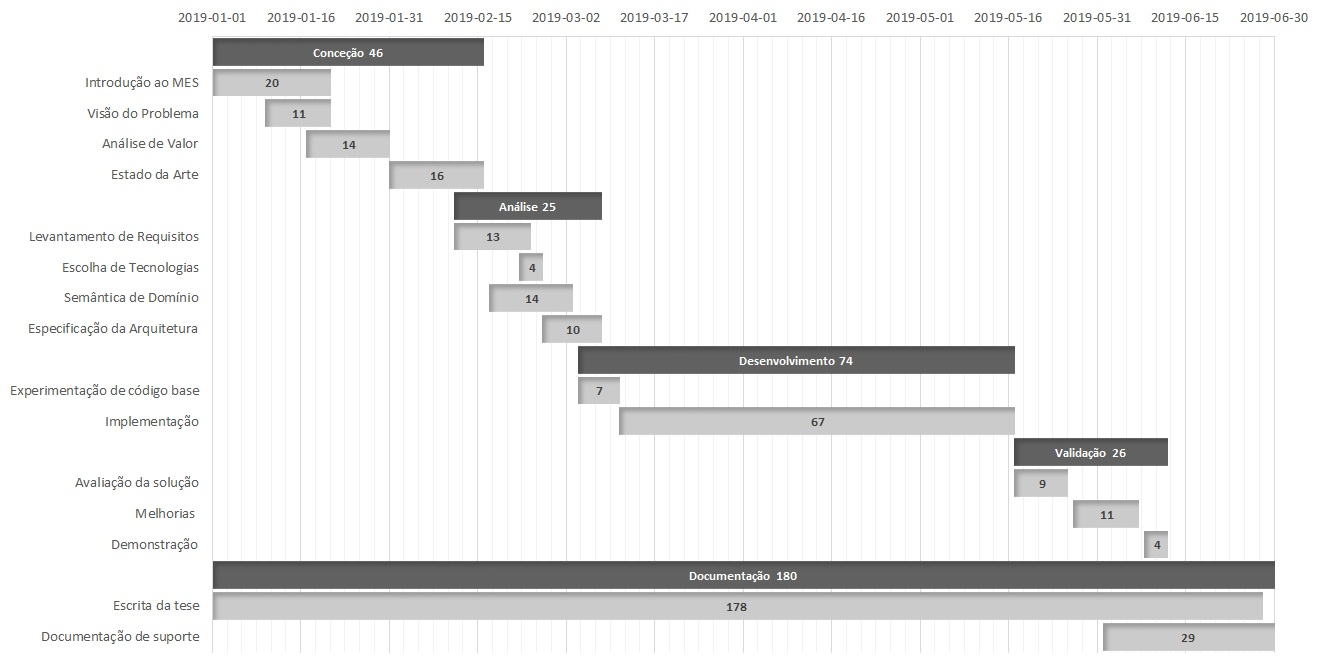
\includegraphics[width=\textwidth]{appendices/assets/gantt.jpg}
    }
    \caption{Diagrama de \textit{Gantt} referente ao planeamento do projeto}
\end{figure}

%\chapter{Análise de Valor}
\label{AppendixB}
Esta capítulo visa a análise da oportunidade de negócio que surge com a nova funcionalidade, cuja abordagem é explorada neste trabalho.

\section{O Processo de Inovação}
De acordo com~\textcite{ffe_effectivemethods_tools_techniques}, o processo de inovação, representado na Figura~\ref{fig:inovation_process}, está dividido em três áreas -- o \gls{ffe}, \gls{npd} e a comercialização -- que correspondem às fases inerentes ao \gls{ncd}, um modelo desenvolvido por um conjunto de empresas, com o objetivo de \inquotes{[...]~fornecer uma linguagem e compreensão comum para as atividades \textit{front end}}\footnote{Tradução livre de autor. No original \inquotes{[...]~to provide a common language and insights on the front end activities.}.}~\parencite{providing_clarity_common_language_ffe}.

O \gls{ffe} representa uma oportunidade para melhoria de todo o processo de inovação, focando todas as atividades que antecedem o desenvolvimento do produto, com o propósito de potenciar o valor, a importância e a probabilidade de sucesso das fases que se seguem. Ou seja, consiste no investimento do tempo em atividades de discussão da ideia, por forma a identificar e estruturar o problema ou oportunidade~\parencite{ffe_effectivemethods_tools_techniques, ffe_theoretical_model}. Porém, as atividades inerentes ao \gls{ffe} são fundamentalmente diferentes da fase \gls{npd}, pelo que se torna necessária a definição de vocabulário específico, permitindo a geração de conhecimento e clara distinção entre as diferentes fases do processo~\parencite{ffe_effectivemethods_tools_techniques}.

\begin{figure}[!ht]
    \centering
    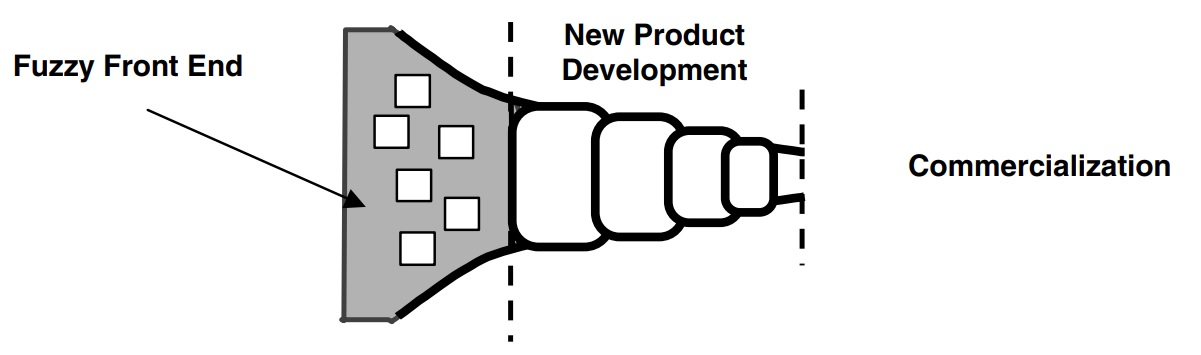
\includegraphics[width=.95\textwidth]{appendices/assets/inovation_process.jpg}
    \caption{O processo de inovação, extraído de~\textcite{ffe_effectivemethods_tools_techniques}}
    \label{fig:inovation_process}
\end{figure}

O modelo \gls{ncd}, demonstrado na Figura~\ref{fig:ncd_model}, baseado num modelo relacional ao invés de um processo linear, visa providenciar uma terminologia para o \gls{ffe}~\parencite{ffe_effectivemethods_tools_techniques}. A área interna define os cinco elementos chave do \textit{Front End of Inovation}: a identificação de oportunidade (\textit{Opportunity Identification}), a análise de oportunidade (\textit{Opportunity Analysis}), a geração e enriquecimento de ideias (\textit{Idea Generation and Enrichment}), a seleção de ideias (\textit{Idea Selection}) e a definição do conceito (\textit{Concept Definition}). O motor central (\textit{Engine}) corresponde à liderança, cultura e estratégia organizacional, que suporta os elementos que compõem o \gls{ffe}, são controláveis pela organização e possibilita a interação entre eles. Já na periferia, encontram-se os fatores de influência (\textit{Influencing Factors}), geralmente incontroláveis pela organização, consistem nas capacidades organizacionais, na estratégia de negócio, no mundo exterior, nomeadamente os canais de distribuição, clientes, fornecedores, concorrentes, política governamental ou legislação, ou quaisquer fatores que possam influenciar todo o processo de inovação~\parencite{ffe_effectivemethods_tools_techniques, providing_clarity_common_language_ffe}.

\begin{figure}[!ht]
    \centering
    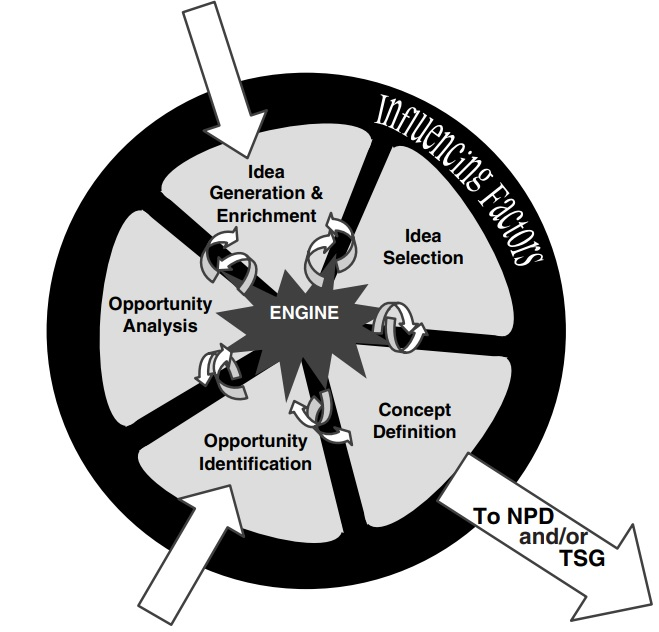
\includegraphics[width=.55\textwidth]{appendices/assets/ncd_model.jpg}
    \caption{A representação do modelo \glsfirst{ncd}, extraído de~\textcite{ffe_effectivemethods_tools_techniques}}
    \label{fig:ncd_model}
\end{figure}

Quanto à representação do modelo, as partes internas são designadas de elementos por oposição a processos, pois estes implicam estrutura, que pode não ser possível ser aplicada. O formato circular indica que é esperado que as ideias fluam, circulem e iterem ao longo dos elementos, por qualquer ordem ou combinação, permitindo o uso dos elementos, repetidamente. Este comportamento é intrínseco às atividades do \gls{ffe}, permitindo uma definição clara do mercado, dos requisitos, dos riscos associados e do plano de negócio, tornando mais eficazes as fases de desenvolvimento e comercialização, devido à redução do tempo total de projeto, fruto da diminuição da repetição de algumas atividades~\parencite{ffe_effectivemethods_tools_techniques}. 

\section{O \textit{Fuzzy Front End} de Inovação}
Como mencionado anteriormente, o \gls{ffe} corresponde a um conjunto de atividades geralmente caóticas, imprevisíveis e não estruturadas que antecedem o desenvolvimento de um produto~\parencite{ffe_incremental_platform_breakthrough_products}. Todavia, é preciso perceber a natureza do produto a desenvolver, de forma a melhor enquadrar o processo de inovação.

Segundo~\textcite{ffe_incremental_platform_breakthrough_products}, pode-se caracterizar os produtos de acordo com a extensão da mudança ou do processo: incremental, requer pouca mudança a nível do produto ou do processo, uma vez que geralmente consiste na redução de custos, melhoria, extensão ou reposicionamento no mercado de produtos já existentes; plataforma, estabelecem uma arquitetura básica para uma nova geração de produtos ou processos; pioneiro, envolve uma mudança significativa no processo ou produto.

O presente trabalho visa o desenvolvimento dum módulo de linguagem natural para o {\productname}, uma plataforma já estabelecida, ou seja, trata-se de uma extensão ao produto já existente, enquadrando-se no tipo incremental. A ideia surge do processo de planeamento estratégico da empresa com a finalidade de trazer novas funcionalidades aos seus clientes, melhorando a qualidade do produto. Portanto, nas secções seguintes, aplica-se a metodologia explicitada, no sentido de enriquecer a proposta de projeto apresentada pela {\companyname}.

\subsection{Identificação da Oportunidade}
O \gls{pln} é uma área de investigação que explora a forma como os computadores podem manipular a linguagem natural (texto ou voz) para executar determinadas tarefas. Aplica-se em diversos campos de estudo: tradução, processamento de texto, interfaces com o utilizador, reconhecimento de voz, sistemas periciais~\parencite{nlp}.

\textcite{end_to_end_neural_nli_databases} menciona que, apesar da expressividade da \gls{sql}, os utilizadores necessitam de algum conhecimento técnico para perceber como extrair informação de um sistema, o que conduziu à investigação para o desenvolvimento de interfaces alternativas que permitam aos utilizadores, sem conhecimento técnico, explorar e interagir com os dados, de forma conveniente. Também \textcite{towards_theory_nli_databases} menciona que a necessidade de interfaces de linguagem natural se torna mais evidente, devido ao número de pessoas sem conhecimentos técnicos que acedem a informação através de \textit{browsers} ou telemóveis, tornando paradigmas como o reconhecimento de voz mais atrativos.

Nesse sentido, a {\companyname} tenciona o desenvolvimento do módulo de linguagem natural para que os utilizadores do produto, sem conhecimento orientado às tecnologias de informação, possam fácil, rápida e intuitivamente consultar o sistema. Desta forma, a funcionalidade destaca o produto pelo uso de novas tecnologias, facilita-se a interação com o sistema, reduzindo-se o tempo de formação técnica associado ao mesmo. 

\subsection{Análise da Oportunidade}
A pesquisa realizada por~\textcite{roadmap_nlp_research_is}, apresentada na Figura~\ref{fig:number_articles_per_year_nlp}, cuja metodologia consistiu na pesquisa de termos como \inquotes{Natural Language Processing} e \inquotes{NLP} em bases de dados académicas, determina que há uma tendência crescente de interesse por esta área. Nos últimos anos, a quantidade de dados textuais disponíveis nas redes sociais ou em sistemas de comunicação, juntamente com a necessidade de acesso a informação, contribuíram para o avanço e adoção comercial do \gls{pln}~\parencite{roadmap_nlp_research_is}.

\begin{figure}[!ht]
    \centering
    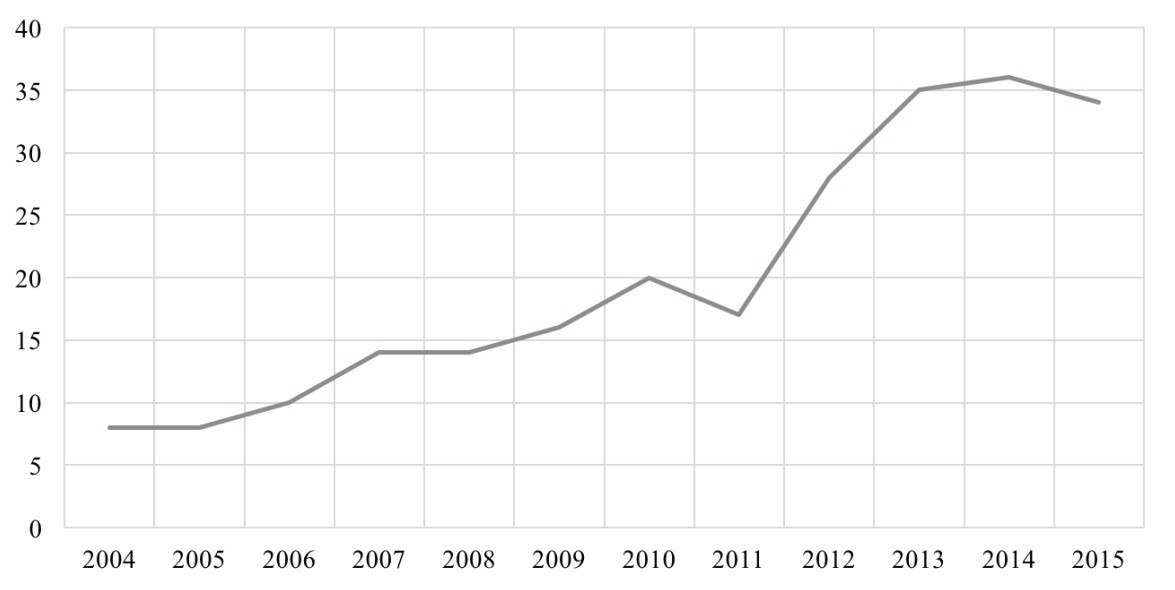
\includegraphics[width=.9\textwidth]{appendices/assets/number_articles_nlp.jpg}
    \caption{Número de artigos de \glsfirst{pln} pesquisados por ano, extraído de~\textcite{roadmap_nlp_research_is}}
    \label{fig:number_articles_per_year_nlp}
\end{figure}

Quanto ao segmento de mercado no qual se integra, cresce a visão de fábricas inteligentes, associadas à quarta revolução industrial, prezando a integração do operador humano num ambiente complexo e rico em dados~\parencite{social_factory}. \textcite{industry40_revolution_future_mes} afirma que a revolução supracitada é já conhecida pelas empresas, o que lhe permite tomar ações no sentido de definir o seu modelo de fabrico e o seu plano de transformação, particularmente na adaptação do \gls{mes} de forma a manter o desempenho, qualidade e agilidade nas desafios espoletados pelas empresas de manufatura. Portanto, a interação entre o ser humano e o sistema pode melhorar o processo de fabrico e potenciar o negócio, na medida em que o operador, em vez do trabalho manual repetitivo que pode facilmente ser automatizado, passa a tomar decisões no processo para resolução de problemas, as quais requerem acesso à informação correta e de forma atempada~\parencite{social_factory}. É nesse sentido que o {\productname} ganha vantagem com o desenvolvimento desta nova funcionalidade.

\subsection{Geração, Enriquecimento e Seleção de Ideias}
No seguimento deste assunto, foram realizadas duas reuniões com o supervisor do projeto na {\companyname}, em que foram discutidos alguns requisitos operacionais e de usabilidade, restrições ao desenvolvimento da solução, como a preferência por uso de ferramentas de \gls{pln} que possam ser mantidas internamente e a sua facilidade de utilização, e ideias para futuras implementações, as quais podem ter um impacto na especificação arquitetural do protótipo.

\begin{figure}
    \centering
    \resizebox{\textwidth}{!}{\begin{tikzpicture}
  \path[mindmap, concept color=black!50,text=white,
    every node/.append style={concept, minimum size=0.5cm, inner sep=0.2mm},
    level 1 concept/.append style={text width=1.5cm,font=\scriptsize},
    level 2 concept/.append style={text width=1.27cm,font=\tiny\bfseries,level distance=50}
  ]
    % Root
    node[text width=2.3cm,font=\small] {Projeto}
    %
    [clockwise from=0]
    child[concept color=black!25,text=black,level distance=80] { node {Restrições}
      [clockwise from=120]
      child { node {Uso Interno} }
      child { node {Custo} }
      child { node {Eficiência} }
      child { node {Aprendizagem da Ferramenta} }
      child { node {Usabilidade da Solução} }
    }
    %
    child[concept color=black!25,text=black,level distance=115] { node {Requisitos}
      [clockwise from=0]
      child { node {Semântica Temporal} }
      child { node {Semântica de Domínio} }
      child { node {Integração com Produto} }
      child { node {Auto-aprendizagem} }
    }
    %
    child[concept color=black!25,text=black,level distance=90] { node {Estado da arte} 
      [clockwise from=-115]
      child { node {Soluções Análogas} }
      child { node {Ferramentas} }
    }
    %
    child[concept color=black!25,text=black,level distance=75] { node {Tecnologia}
      [counterclockwise from=75]
      child { node {PLN} }
      child { node {Interfaces de Linguagem Natural} }
      child { node {\textit{Data Warehouses}} }
    }
    %
    child[concept color=black!25,text=black,level distance=125] { node {Clientes}
      [counterclockwise from=-30]
      child { node {Semi\\condutores} }
      child { node {Equipamentos Médicos} }
      child { node {Montagem Eletrónica} }
      child { node {Energia Solar} }
      child { node {Outros} }
    }
    child[concept color=black!25,text=black,level distance=135] { node {Utilizadores}
      [counterclockwise from=-35]
      child { node {Engenheiros de Produção} }
      child { node {Engenheiros de Qualidade} }
      child { node {Responsáveis de Linha} }
      child { node {Operadores} }
    };
\end{tikzpicture}}
    \caption{\textit{Mindmap} das ideias e conceitos gerados}
    \label{fig:mindmap}
\end{figure}

Em relação às ideias e conceitos contempladas no \textit{mindmap} da Figura~\ref{fig:mindmap}, o presente projeto pretende dar resposta a praticamente todos, tendo em consideração que, numa fase inicial, o cumprimento de todos é praticamente inatingível. A descrição de cada conceito é feito de seguida:

\begin{itemize}
    \item
    {
        \textit{Tecnologia} -- a ideia inerente ao trabalho assenta sobre as temáticas de \gls{pln}, especificamente Interfaces de Linguagem Natural, e \textit{Data Warehouses}. Esta consiste no estudo aprofundado deste tipo de interfaces orientado à consulta em armazéns de dados e disseminação do conhecimento internamente, para que no futuro, o projeto possa ter continuidade;
    }
    \item
    {
        \textit{Estado da Arte} -- abordagem de ferramentas e soluções análogas, com o objetivo de especificar uma arquitetura para o sistema. Este processo dá origem aos documentos de especificação que devem ser usados para consulta por parte dos desenvolvedores, quer numa perspetiva de conhecimento arquitetural, quer das ferramentas que são usadas;
    }
    \item
    {
        \textit{Clientes} -- uma vez que a {\companyname} possui clientes com diferentes realidades, a ideia é que o módulo final esteja preparado para elaborar consultas em qualquer domínio, de forma configurada ou cerne da solução. Contudo, como já abordado anteriormente, no contexto deste trabalho, apenas um domínio será considerado;
    }
    \item
    {
        \textit{Utilizadores} -- a solução deverá responder às necessidades de qualquer utilizador, desde os mais técnicos (Engenheiros de Produção) aos menos técnicos (Operadores). Porém, o protótipo terá em consideração os utilizadores mais comuns do {\productname};
    }
    \item
    {
        \textit{Restrições} -- nesta temática, foram discutidas alternativas como a avaliação do custo de uma ferramenta proprietária, uso de ferramentas \textit{open source} ou o desenvolvimento interno da própria biblioteca de \gls{pln}, de modo a garantir que não existem dependências externas à plataforma. Também foram discutidas a eficiência da solução em contexto produtivo, a facilidade de aprendizagem e usabilidade da mesma. Assim, a usabilidade do módulo de linguagem natural será estudada a partir do mecanismo de \textit{feedback} provido na solução e através de inquéritos aos utilizadores, o que também se aplica para a aprendizagem da ferramenta. Relativamente aos restantes tópicos, não houve conclusão acerca das ideias a serem selecionadas;
    }
    \item
    {
        \textit{Requisitos} -- pressupõe-se o uso de auto-aprendizagem para adaptação automática do módulo ao \textit{feedback} do utilizador, ainda que para o protótipo, a resposta a uma simples pergunta como \inquotes{A resposta obtida foi-lhe útil?} é suficiente. Também a integração com o produto, quer a nível aplicacional, quer a nível de processo deve ser considerada, o que resultará na organização de \textit{meetups} com as equipas responsáveis pelo processo de manutenção da plataforma. Quanto aos restantes conceitos, não houve conclusão acerca das ideias selecionadas.
    }
\end{itemize}

\subsection{Definição do Conceito}
Todo o processo presente no modelo \gls{ncd} de \gls{ffe} culmina com a definição do conceito, a fase que encaminha o projeto para a implementação~\parencite{ffe_effectivemethods_tools_techniques}.

O presente trabalho, denominado de \inquotes{Natural Language Querying} consiste no desenvolvimento de um protótipo de um módulo de linguagem natural e definição de uma abordagem que será tida em conta no módulo final para interface com o {\productname}. Esse módulo final permitirá a consulta e pesquisa de estados do processo de fabrico por utilizadores com pouco ou nenhum conhecimento associado a tecnologias de informação, garantindo a interação com o sistema de uma forma simples, fácil e intuitiva, melhorando o processo numa perspetiva de apoio à decisão (ver Secção~\ref{sec:chap01_problem}). Os objetivos deste projeto estão descritos na Secção~\ref{sec:chap01_objectives}, a metodologia e critérios de sucesso na Secção~\ref{sec:chap01_solutionevaluation}, e o respetivo plano de trabalho no Capítulo~\ref{sec:chap01_workmethodology}.

O projeto traz benefícios para a empresa e o seu produto, pelo estudo e adoção de tecnologia de \gls{pln} num contexto industrial, pela possível melhoria de usabilidade do sistema e pela evolução no processo de apoio à decisão dos seus clientes. Uma vez que o {\productname} é um produto bem posicionado no mercado, não se esperam riscos a nível comercial. Contudo, a uso de tecnologia recente, cujos conceitos não estão totalmente estudados e cujos trabalhos de investigação são limitados, pode provocar atrasos no desenvolvimento do projeto ou incumprimento do orçamento definido. Não obstante, o projeto avança com o desenvolvimento de um protótipo, fase que decidirá a inclusão do módulo na plataforma da {\companyname}.


%\chapter{Protótipo}
\label{AppendixC}
Neste apêndice são mostrados alguns artefactos recolhidos ao longo das fases de conceção, desenvolvimento e validação do protótipo.

\section{Configuração}
Nesta secção apresentam-se algumas imagens referentes ao processo de configuração levado no protótipo.
%
\begin{figure}[!ht]
    \centering
    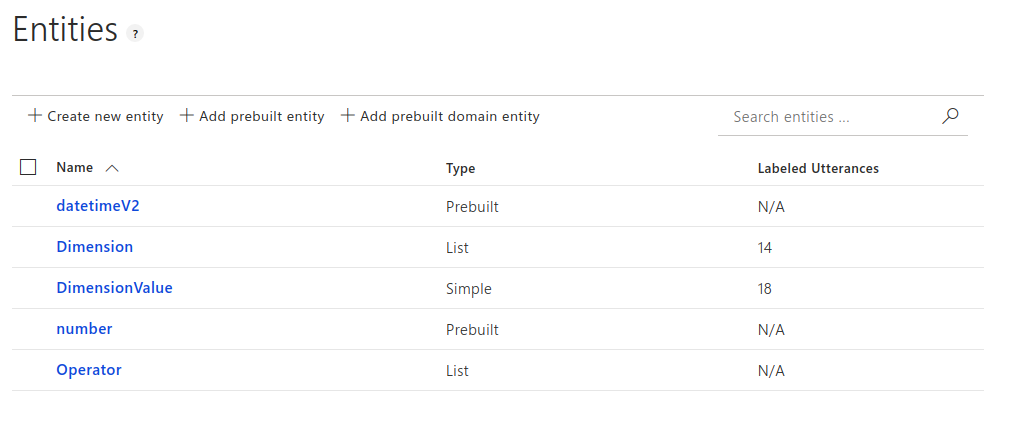
\includegraphics[width=\textwidth]{appendices/assets/kb07.png}
    \caption{Definição das entidades esperadas}
\end{figure}
%
\begin{figure}
\centering
    \begin{subfigure}{.9\textwidth}
        \centering
        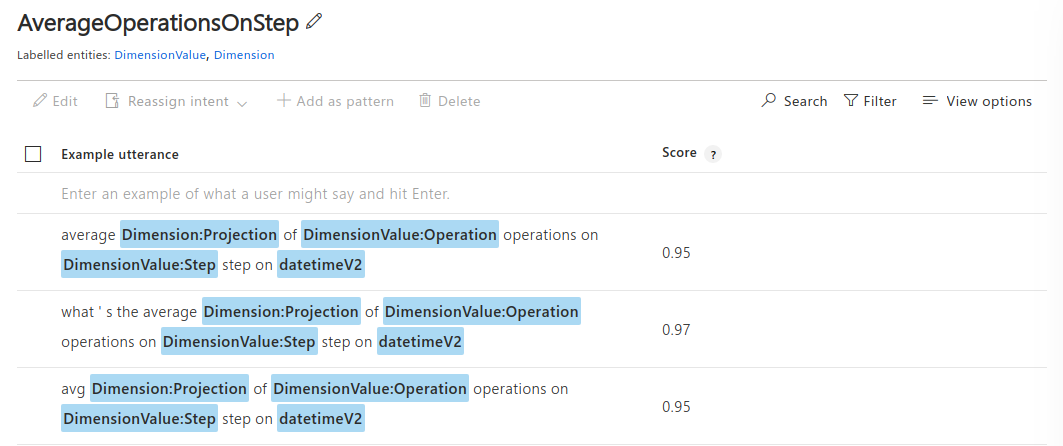
\includegraphics[width=\textwidth]{appendices/assets/kb01.png}
        \caption{Intenção \textit{AverageOperationOnStep}}
     \end{subfigure}
     \begin{subfigure}{.9\textwidth}
         \centering
        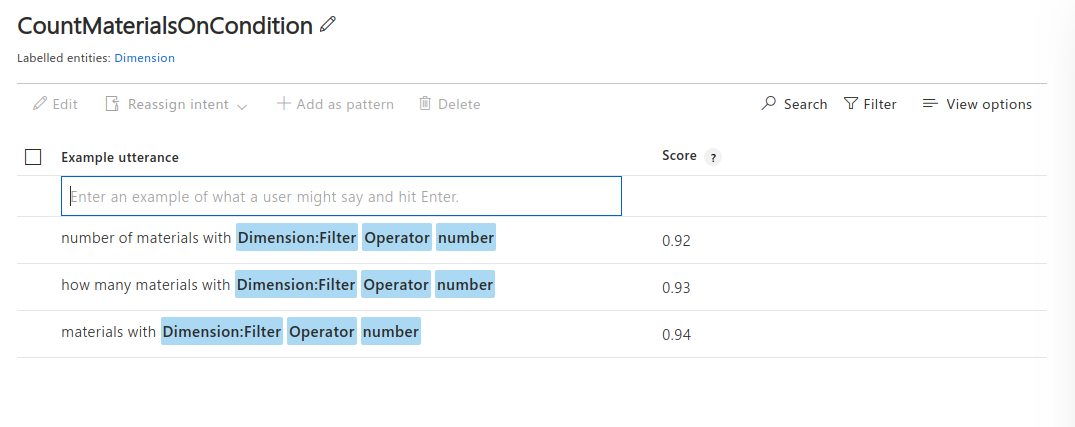
\includegraphics[width=\textwidth]{appendices/assets/kb02.png}
        \caption{Intenção \textit{CountMaterialsOnCondition}}
     \end{subfigure}
     \begin{subfigure}{.9\textwidth}
        \centering
        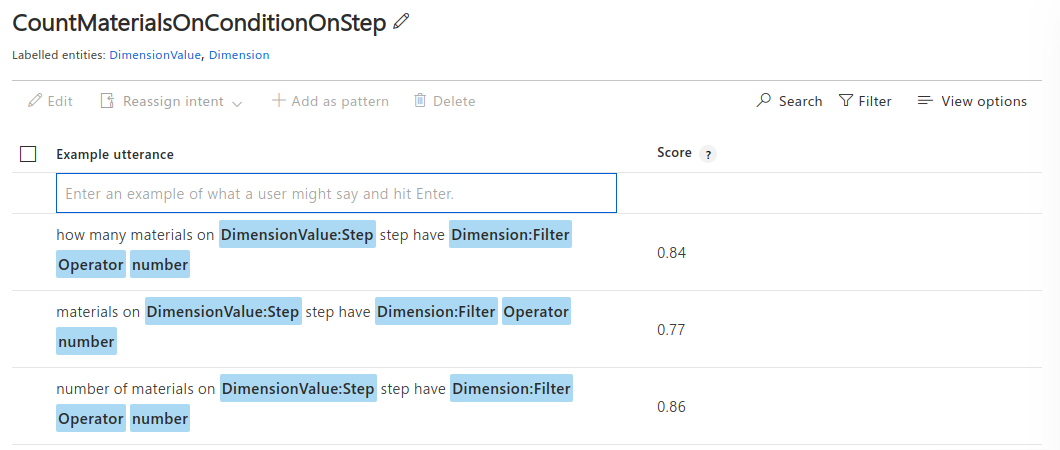
\includegraphics[width=\textwidth]{appendices/assets/kb03.png}
        \caption{Intenção \textit{CountMaterialsOnConditionOnStep}}
     \end{subfigure}
\caption{Intenções definidas, contendo as expressões e respetivas entidades}
\end{figure}
%
\begin{figure}
    \centering
         \begin{subfigure}{.9\textwidth}
        \centering
        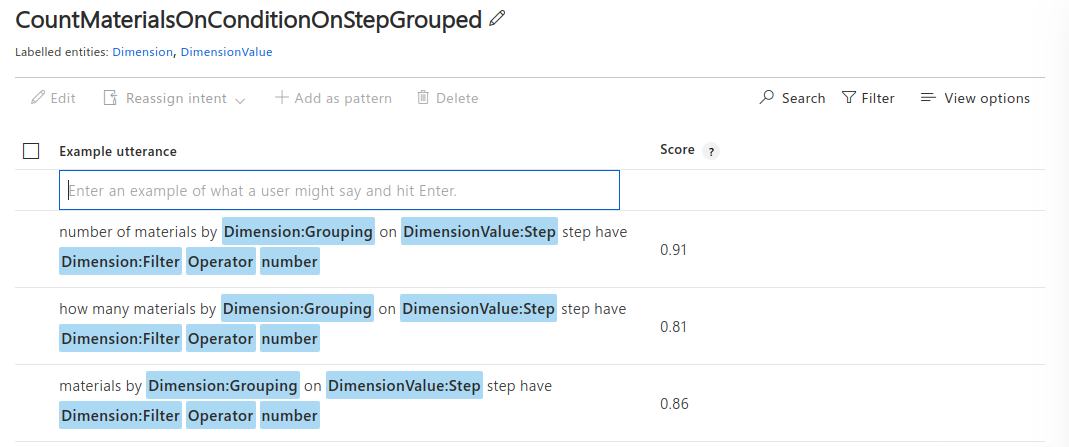
\includegraphics[width=\textwidth]{appendices/assets/kb04.png}
        \caption{Intenção \textit{CountMaterialsOnConditionOnStepGrouped}}
     \end{subfigure}
     \begin{subfigure}{.9\textwidth}
        \centering
        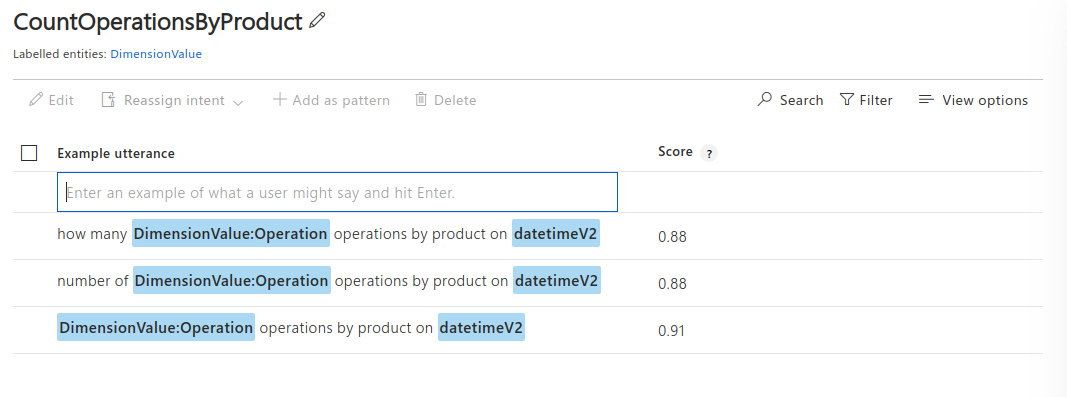
\includegraphics[width=\textwidth]{appendices/assets/kb05.png}
        \caption{Intenção \textit{CountOperationsByProduct}}
     \end{subfigure}
     \begin{subfigure}{.9\textwidth}
        \centering
        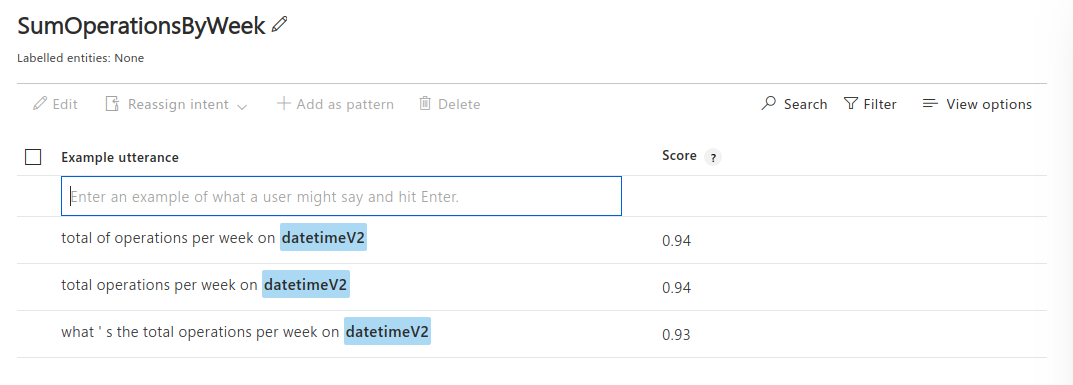
\includegraphics[width=\textwidth]{appendices/assets/kb06.png}
        \caption{Intenção \textit{SumOperationsByWeek}}
     \end{subfigure}
    \caption{Continuação das intenções definidas, contendo as expressões e respetivas entidades}
\end{figure}

\clearpage

\section{Validação}
Nesta secção apresentam-se algumas imagens referentes ao processo de validação do protótipo.

\begin{figure}[!ht]
\centering
    \begin{subfigure}{.48\textwidth}
        \centering
        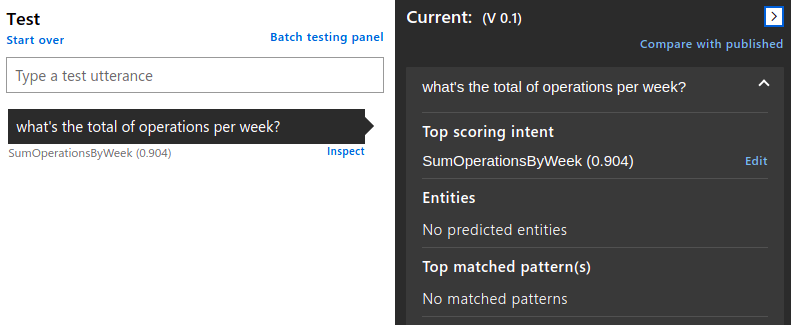
\includegraphics[width=\textwidth]{appendices/assets/nlcomprehension01.png}
        \caption{Intenção \textit{SumOperationsByWeek}}
     \end{subfigure}
     \begin{subfigure}{.48\textwidth}
         \centering
        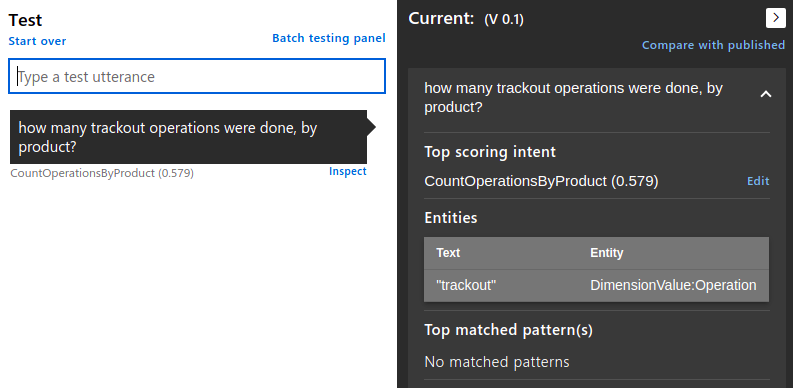
\includegraphics[width=\textwidth]{appendices/assets/nlcomprehension02.png}
        \caption{Intenção \textit{CountOperationByProduct}}
     \end{subfigure}
     \bigbreak
     \begin{subfigure}{.48\textwidth}
        \centering
        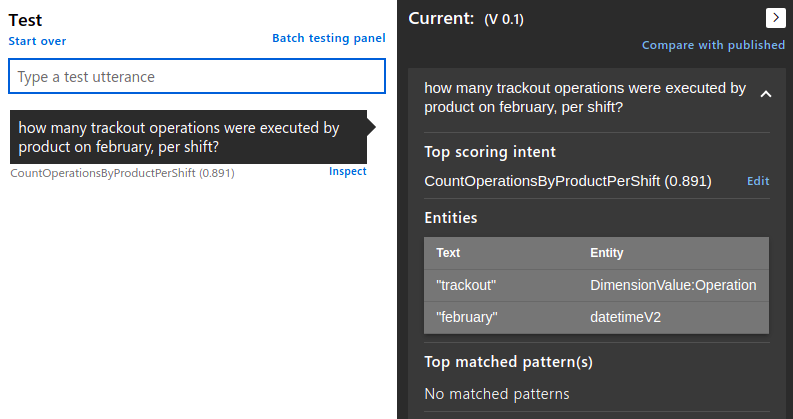
\includegraphics[width=\textwidth]{appendices/assets/nlcomprehension03.png}
        \caption{Intenção \textit{AverageOperationsOnStep}}
     \end{subfigure}
     \begin{subfigure}{.48\textwidth}
        \centering
        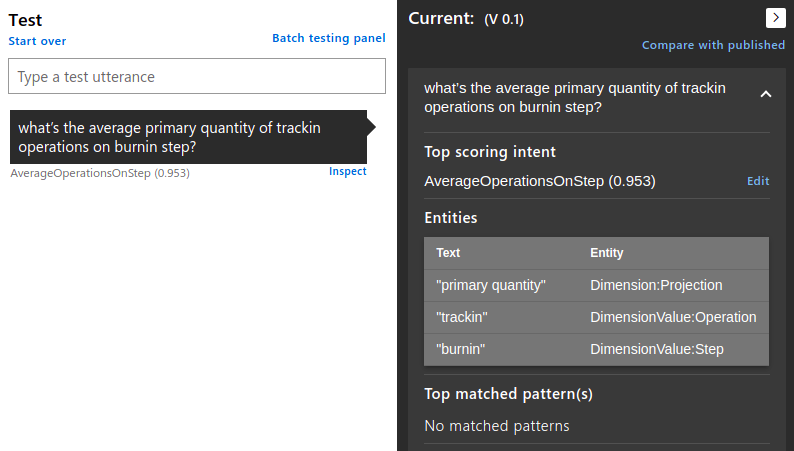
\includegraphics[width=\textwidth]{appendices/assets/nlcomprehension04.png}
        \caption{Intenção \textit{CountOperationsOnConditionOnStepGrouped}}
     \end{subfigure}
     \bigbreak
     \begin{subfigure}{.48\textwidth}
        \centering
        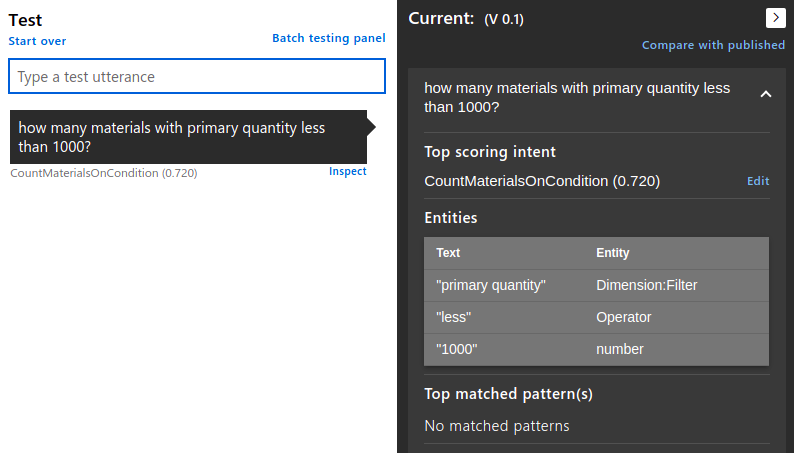
\includegraphics[width=\textwidth]{appendices/assets/nlcomprehension05.png}
        \caption{Intenção \textit{AverageOperationsOnStep}}
     \end{subfigure}
     \begin{subfigure}{.48\textwidth}
        \centering
        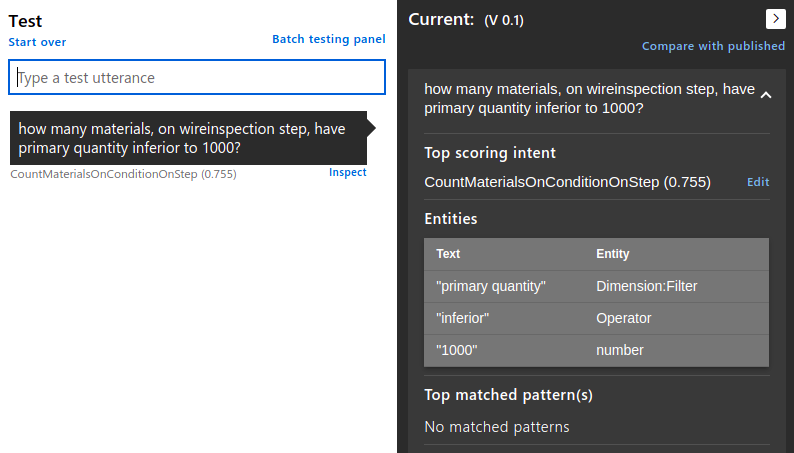
\includegraphics[width=\textwidth]{appendices/assets/nlcomprehension06.png}
        \caption{Intenção \textit{CountOperationsOnConditionOnStepGrouped}}
     \end{subfigure}
\caption{Outras imagens relativas à avaliação de intenções e entidades do protótipo}
\label{fig:nlcomprehesion_others}
\end{figure}

%----------------------------------------------------------------------------------------

\end{document}
